\section{Options flowchart and explanation~\ref{fig:options}}

\begin{figure}
    \centering 
    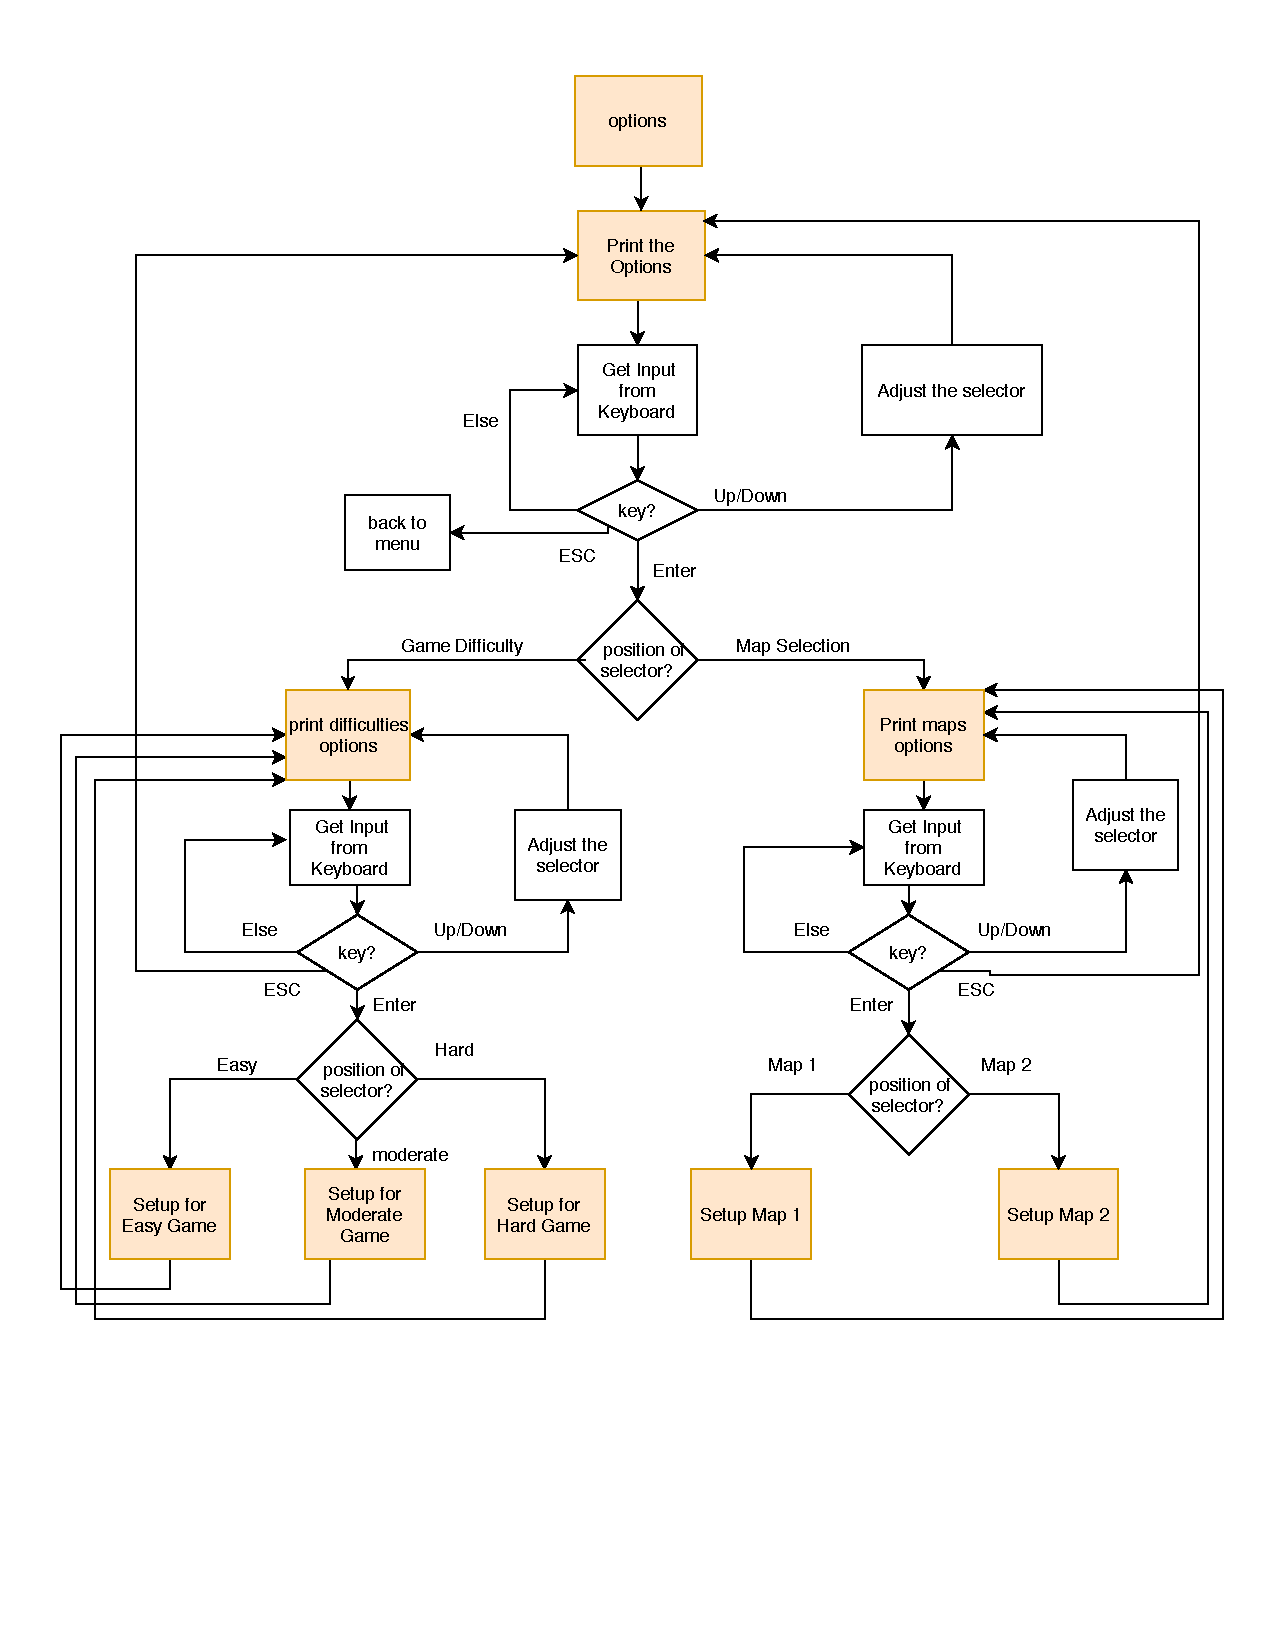
\includegraphics[width=\columnwidth]{options.pdf}
    \caption{Options block flowchart. Blocks which are in \textcolor{orange}{orange} will be implemented for the second release. Some functions and blocks are used in both menu and options which are in white color.}
    \label{fig:options}
\end{figure}


This flow chart explains all the steps happening on the options block. 
As it is shown in Figure~\ref{fig:options} initially, options items which are map selection and game difficulty are printed for the user. 
Next, according to the user input key the program goes to one of the following states: 
back to menu, adjust the selector, choose between map selection, or game difficulty, and read another input. 
A selector is placed besides each option item; the player can see the selector and is informed on its selection.
Similarly, some items will be printed for game difficulties and available maps and the user is able to choose from them.
In each stage escape key goes to the previous stage and enter key chooses and option. 
The selected difficulty and map will be used to do the single-player and multi-player setup later.

\subsection{Options functions prototypes}

In this section we define the required functions prototypes and its relation to flow chart~\ref{fig:options}.

\begin{minted}{c}

#define OPTION_ITEM_MAX_SIZE 1000
#define OPTION_NUM_ITEMS 2
#define OPTION_NUM_MAPS 2
#define OPTION_NUM_DIFFICAULTIES 3

typedef enum 
{
    OPTION_TOP,
    OPTION_DIFFICAULTY,
    OPTION_MAP,
} OptionMenues;

typedef struct OptionItem {
    char str[OPTION_ITEM_MAX_SIZE];
} OptionItem;

typedef struct Option {
    int selector;
    int difficualtySelector;
    int mapSelector;
    OptionItem items[OPTION_NUM_ITEMS]
    OptionItem difficaultyItems[OPTION_NUM_DIFFICAULTIES];
    OptionItem mapItems[OPTION_NUM_ITEMS];
    OptionMenues optionMenu;
    FILE* configFile;
} Option;

void backToMenu(void);

/* Block: Print the options - second release
 * Assigned to:
 * Prints the options' items on the console.
 * Input: option
 * Return: void */
void printOptions(Option* option_p);

/* Block: update the selector - second release
 * Assigned to:
 * Updates the selector position according to input key.
 * Input: option_p, arrowKey
 * Output: option_p
 * Return: void*/
void updateSelector(Option* option_p, int arrowkey);

/* Block: update the selector - second release
 * Assigned to:
 * This will call functions related to each option
 * Input: selector
 * Output: 
 * Return: void*/
void chooseMenuOption(OptionMenues optionMenu);

/* Block: Setup for easy/moderate/hard game - second release
 * Assigned to:
 * select a difficulty level
 * Input: option, key
 * Output: difficulty level
 * Return: int */
void setDifficulty(Option option_p, int key);

/* Block: Setup map 1/2 - second release
 * Assigned to:
 * select a map
 * Input: option, key
 * Output: map number
 * Return: int */
int setMap(Option* option_p, int key);

\end{minted}